\section{Results}
\begin{figure*}
\begin{tabular}{ l l l l l l l l l }
 scenario & \#obstacles & world size & path length & \#segsments & Theta* time & GA time & MILP time & score \\ 
 \hline
Up/Down Small & 5 &  25m x 20m & 88m  & 7 & 0.09s & 1.10s & 20.8s & 26.6s\\
Up/Down Large & 9 & 40m x 20m &  146m & 11 & 0.14s & 1.62s & 40.1s & 43.6s \\
SF Small & 684 & 1km x 1km & 1392m & 28 & 2.04s & 9.56s & 59.2s & 105.7s \\
SF Large & 6580 & 3km x 3km & 4325m  & 84 & 18.14s & 18.21s & 231s & 316.0s\\
Leuven Small & 3079 & 1km x 1km & 1312m & 29 &  2.29s & 29.83s & 152s  & 95.9s \\
Leuven Large & 18876 & 3km x 3km & 3041m & 61 & 18.14s & 83.69s & 687s & 217.6s \\

\end{tabular}
\caption{The experimental results for the different scenarios}
\label{table:results}
\end{figure*}

\begin{figure}
\begin{tabular}{ l  r | l r }
grid size 			& $2m$ 	& turn tolerance 		& $2$ \\
approach multiplier & $2$ 	& population size 		& $ 10$ \\
\# generations 		& $25$ 	& max. nudge distance 	& $5m$\\
min. \# vertices 	& $ 4$ 	& max. \# vertices 		& $12$ \\
P(add vertex) 		& $0.1$ & P(remove vertex) 		& $0.1$  \\
max nudge attempts 	& $15$ 	& $ T_{max}$ 			& $5s$ \\
time step size 		& $0.2s$& &
%approach margin, maxsegment time
%fps
%pop, gens, mutrate, nudge dist, minpoints-maxpoints, addprob, removeprob
\end{tabular}
\caption{The parameters used for testing}
\label{table:params}
\end{figure}

\begin{figure}
	\centering
	
	\begin{subfigure}[t]{0.7\columnwidth}
        		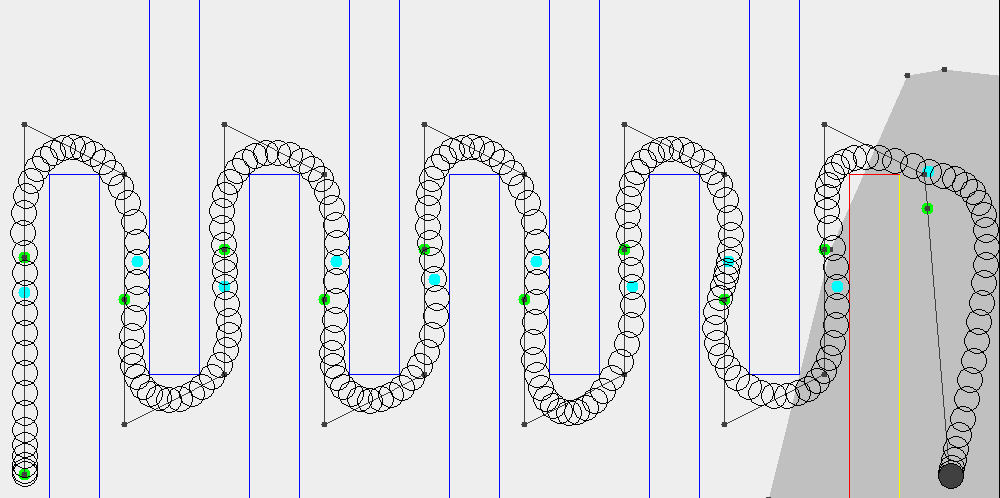
\includegraphics[width=\textwidth]{img/benchmarkfull}
        		\caption{Up/Down Scenario}
        		\label{fig:scen-updown}
	\end{subfigure}
	\par\bigskip
	\begin{subfigure}[t]{0.38\columnwidth}
        		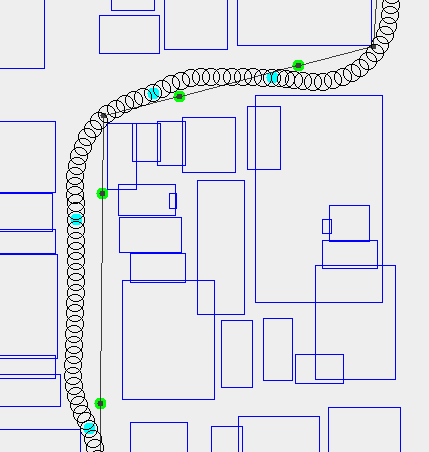
\includegraphics[width=\textwidth]{img/SF_zoom}
        		\caption{A small part of the San Francisco Scenario}
        		 \label{fig:scen-sf}
	\end{subfigure}	
		\hfil
	\begin{subfigure}[t]{0.38\columnwidth}
        		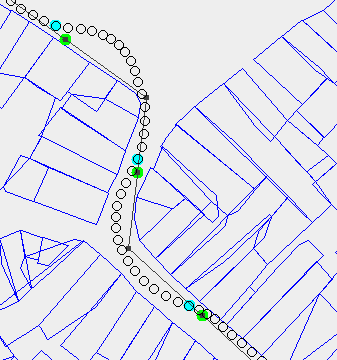
\includegraphics[width=\textwidth]{img/leuven_zoom}
        		\caption{A small part of the Leuven Scenario}
        		\label{fig:scen-leuven}
	\end{subfigure}
        
    \caption{}\label{fig:scenarios}
\end{figure}
We test our algorithm in several different scenarios. Each scenario was tested with two different problem sizes. All tests were executed on an Intel Core i5-4690K running at 4.4GHz with 16GB of 1600MHz DDR3 memory. The reported times are averages of 5 runs. The machine runs on Windows 10 using version 12.6 of IBM CPLEX. Fig. \ref{fig:scenarios} shows these scenarios visually. Fig. \ref{table:results} shows a table with detailed information about the scenarios and execution times. Fig. \ref{table:params} shows the parameters used in the execution of the algorithm.

\subsection{Up/Down Scenario}
The first test scenario has very few obstacles, but lays them out in a way such that the UAV needs to slalom around them. The small scenario has only 5 obstacles, while the larger one has 9. Fig. \ref{fig:scen-updown} shows the large variant. This is a challenging scenario for MILP because every obstacle causes a turn, making the problem significantly less convex. Without segmentation on the small version of the scenario, the solver does not find the optimal trajectory within 30 minutes. If execution is limited to 10 minutes, the best trajectory it finds takes 26.0s to execute by the UAV. That is less than a second faster than the segmented result while it took more than 20 times more execution time to find that trajectory. For the larger scenario with 9 obstacles, the solver could not find a trajectory within 30 minutes. This scenario clearly shows the advantages of segmentation, even if there only are a few obstacles.

\subsection{San Francisco Scenario}
The San Francisco scenario covers a 1km by 1km section of the city for the small scenario, and 3km by 3km section for the large scenario. Fig. \ref{fig:scen-sf} shows the small variant. All the obstacles in this scenario are grid-aligned rectangles laid out in typical city blocks. Because of this, density of obstacles is predictable. This scenario showcases that the algorithm can scale to realistic scenarios with much more obstacles than is typically possible with a MIP approach. 

\subsection{Leuven Scenario}
The Leuven scenario also covers both a 1km by 1km and 3km by 3km section, this time of the Belgian city of Leuven. This is an old city with a very irregular layout. The dataset, provided by the local government\footnote{\url{https://overheid.vlaanderen.be/producten-diensten/basiskaart-vlaanderen-grb}}, also contains full polygons instead of the grid-aligned rectangles of the San Francisco dataset. While most buildings in the city are low enough so a UAV could fly over, it presents a very difficult test case for the trajectory planning algorithm. The density of obstacles varies greatly and is on average much higher than in the San Francisco dataset. The algorithm does slow down compared to the San Francisco dataset, but still runs in an acceptable amount of time. As visible in Fig. \ref{fig:scen-leuven}, there are many obstacles clustered close to each other, with many edges being completely redundant. For a real application, a small amount of preprocessing of the map data should be able to significantly reduce both the amount of obstacles as the amount of edges. 

\section{Conclusion}
Path planning using MIP was previously not computationally possible in large and complex environments. The approach presented in this paper shows that these limitations can effectively be circumvented by dividing the path into smaller segments using several steps of preprocessing. The final trajectory is generated by a solver so the constraints on the trajectory can easily be changed to account for different use cases. The experimental results show that the algorithm works well in realistic, city-scale scenarios, even when obstacles are distributed irregularly and dense.\\
We demonstrate that our new approach can be used to improve the scalability of MILP trajectory planning. However, more work is required to use the algorithm with an actual UAV.  Extending the algorithm to 3D is the next step. A complimentary, short-term online planner is necessary for a physical UAV to execute the generated trajectory.